\documentclass[11pt,a4paper]{article}

\usepackage[T1]{fontenc}
\usepackage[utf8]{inputenc}
\usepackage[main=french,provide=*]{babel}
\usepackage{lmodern}
\usepackage[a4paper,margin=2.1cm]{geometry}
\usepackage{graphicx}
\usepackage{booktabs}
\usepackage{array}
\usepackage{tabularx}
\usepackage{float}
\usepackage{xcolor}
\usepackage{hyperref}

\hypersetup{
  colorlinks=true,
  linkcolor=black,
  urlcolor=blue,
  pdftitle={Note Produit - Moteur d'Analyse Technique et Dashboard},
  pdfauthor={Taha Dazine}
}

\setlength{\parindent}{0pt}
\setlength{\parskip}{0.5em}
\renewcommand{\arraystretch}{1.15}

\begin{document}
\pagenumbering{gobble}

\begin{titlepage}
\centering
\vspace*{1.6cm}

{\Huge \bfseries Note Produit\par}
\vspace{0.25cm}
{\LARGE \bfseries Moteur d'Analyse Technique\\[0.15cm] et Dashboard de Signaux\par}
\vspace{0.7cm}
{\large Support de présentation à destination du desk\par}

\vspace{1.0cm}
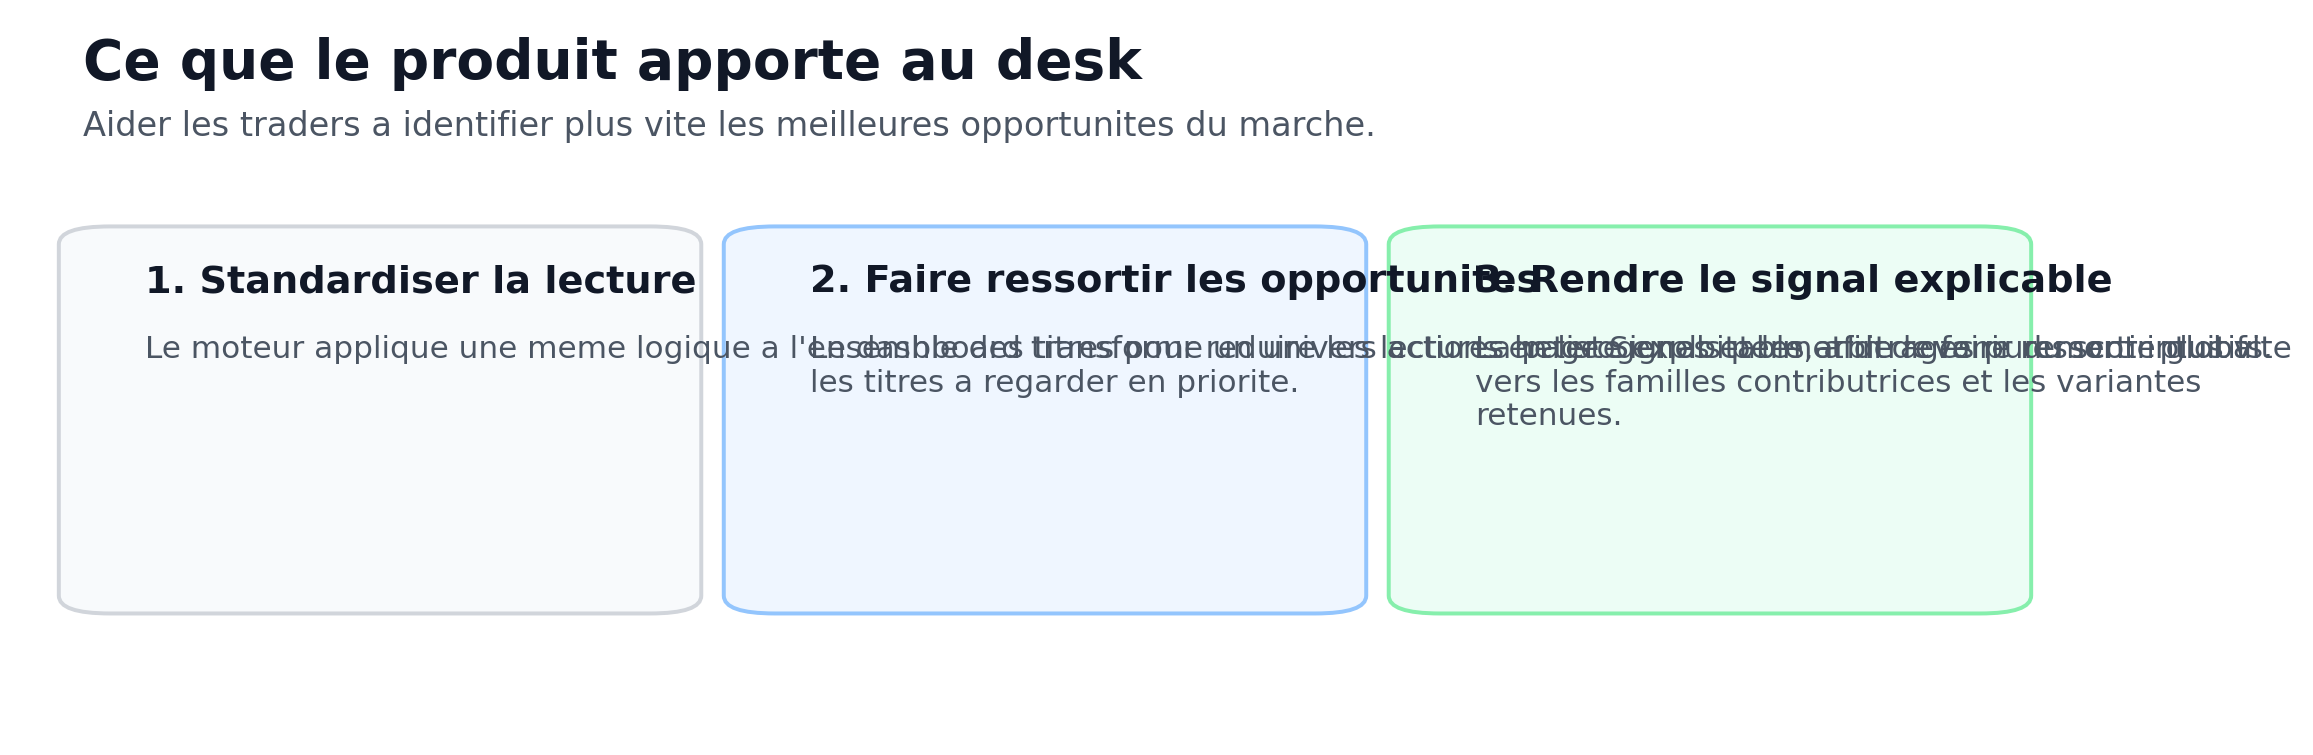
\includegraphics[width=0.97\textwidth]{figures/desk_signal_exec/value_prop.png}

\vspace{1.0cm}
\begin{minipage}{0.92\textwidth}
\large
Cette solution a été développée dans le cadre d'un stage, avec une ambition très simple : \textbf{aider les traders du desk à trouver les meilleures opportunités du marché}. Le produit ne remplace pas la décision humaine. Il rend la lecture technique plus claire, plus rapide et plus exploitable.
\end{minipage}

\vfill
\fcolorbox{black}{gray!8}{
\parbox{0.9\textwidth}{
\centering
\textbf{Périmètre présenté}\\
OHLCV canonique \textrightarrow{} Signal Engine \textrightarrow{} page Signals \textrightarrow{} Dashboard V1
}}

\vspace{0.8cm}
{\large Avril 2026\par}
\end{titlepage}

\clearpage
\pagenumbering{arabic}

\section*{1. L'enjeu métier}

Sur un desk actions, l'enjeu n'est pas seulement de produire de la lecture technique. L'enjeu est surtout de \textbf{repérer rapidement les meilleures opportunités du marché}.

En pratique, l'information disponible est abondante : plusieurs titres, plusieurs horizons, plusieurs indicateurs, parfois plusieurs messages contradictoires. Sans cadre produit clair, le trader voit beaucoup de signaux, mais il ne voit pas toujours immédiatement quels dossiers méritent réellement son attention.

Le produit présenté répond à ce problème de manière concrète :

\begin{itemize}
\item il \textbf{fait ressortir} les titres les plus intéressants à un horizon donné ;
\item il \textbf{structure} la lecture par titre, par famille et par horizon ;
\item il \textbf{donne une justification} au signal pour renforcer la confiance dans la lecture.
\end{itemize}

L'objectif n'est donc pas de couvrir tout le processus d'investissement. L'objectif est plus simple et plus opérationnel : \textbf{aider les traders du desk à trouver plus vite les meilleures opportunités du marché}, puis à comprendre rapidement pourquoi elles ressortent.

\section*{2. Le produit, simplement}

Le produit repose sur deux surfaces complémentaires.

\begin{figure}[H]
\centering
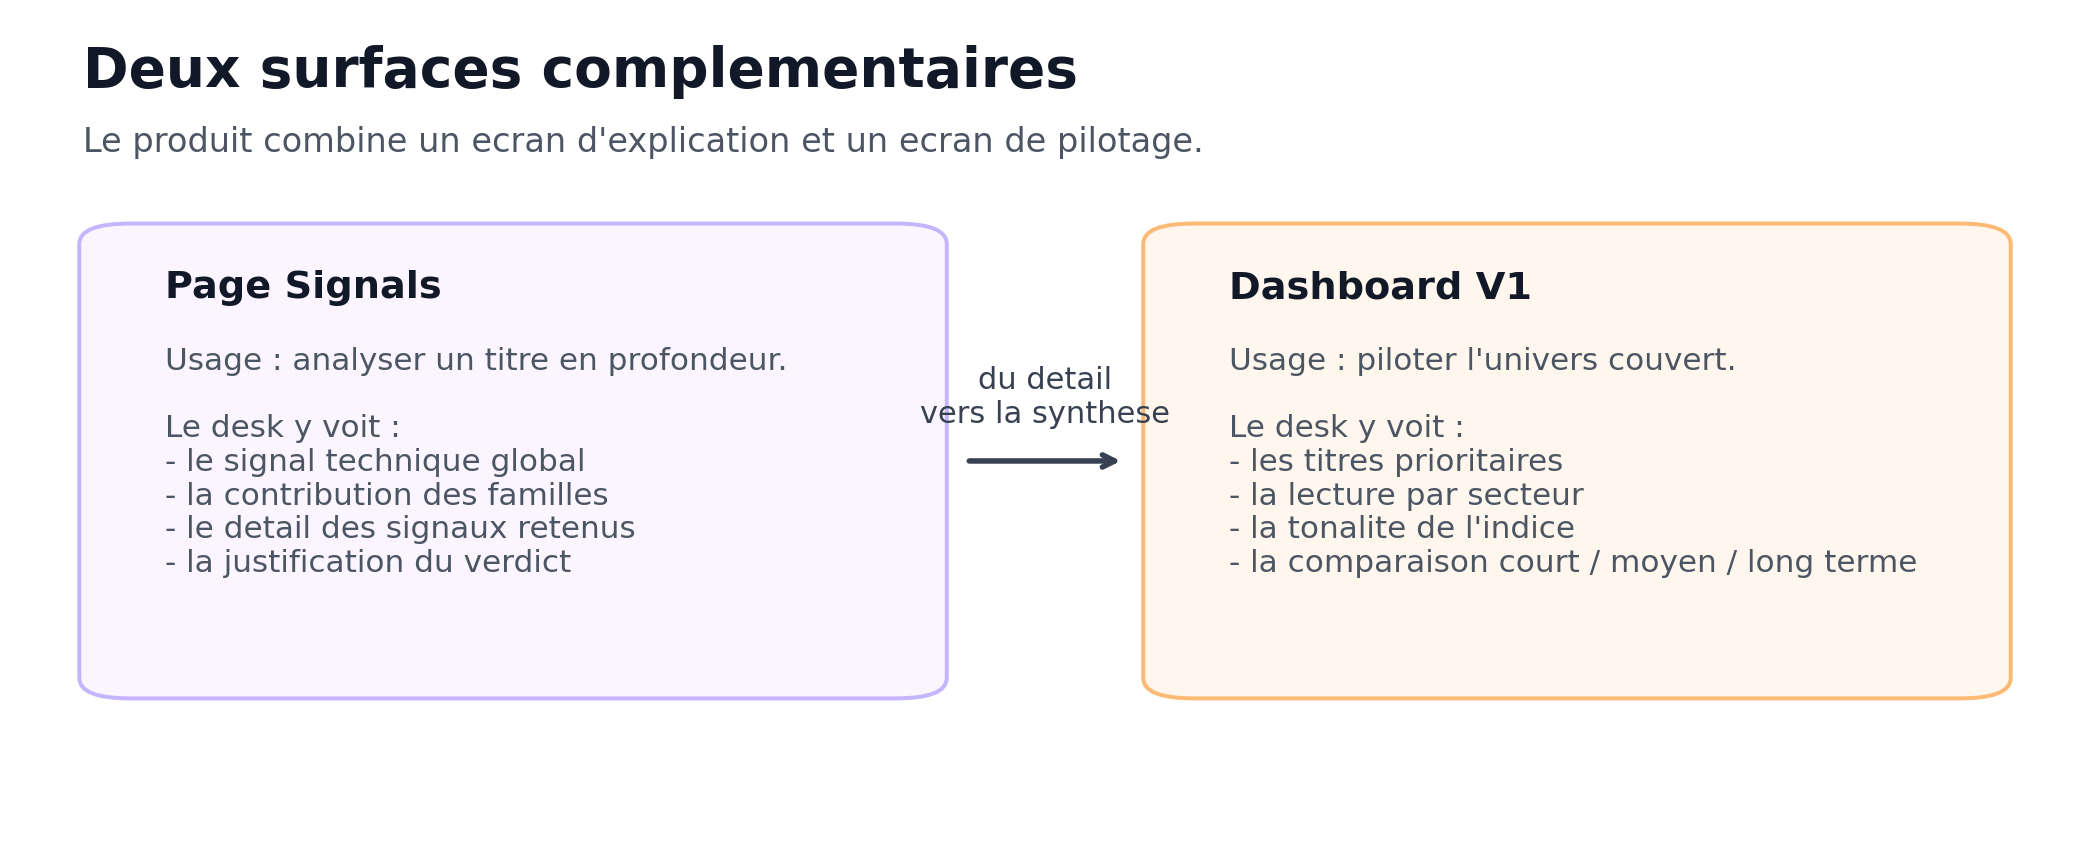
\includegraphics[width=\textwidth]{figures/desk_signal_exec/product_surfaces.png}
\caption{Positionnement fonctionnel des deux surfaces produit.}
\end{figure}

\textbf{La page Signals} est l'écran d'explication. Elle permet d'ouvrir un titre, de lire son signal technique global, puis de comprendre quelles familles contribuent réellement au message final.

\textbf{Le dashboard V1} est l'écran de synthèse. Il permet au desk de parcourir l'univers, de repérer les titres qui ressortent, de comparer les secteurs, de lire la tonalité de l'indice et de distinguer plusieurs horizons d'analyse.

Le socle mis en avant dans cette présentation repose sur \textbf{quatre familles cœur} :

\begin{itemize}
\item \textbf{SMA} pour la tendance ;
\item \textbf{MACD} pour le momentum ;
\item \textbf{RSI} pour l'oscillation ;
\item \textbf{OBV} pour le volume.
\end{itemize}

Ce choix est volontairement lisible. Il couvre plusieurs angles de lecture tout en gardant une restitution exploitable pour un public métier.

\section*{3. Ce que fait le moteur}

Le moteur applique un pipeline de sélection et d'agrégation à plusieurs variantes d'indicateurs. L'idée n'est pas de retenir le paramètre qui ``a le mieux marché'' sur le passé, mais de faire remonter au desk les opportunités les plus crédibles.

En termes de produit, cela se traduit par quatre bénéfices concrets :

\begin{itemize}
\item la lecture finale est \textbf{moins arbitraire} ;
\item les signaux faibles ou trop fragiles sont \textbf{filtrés} ;
\item les signaux quasi identiques ne sont pas comptés plusieurs fois ;
\item le résultat final reste \textbf{synthétique et explicable}.
\end{itemize}

Le moteur aboutit à un score global simple à lire, tout en conservant la possibilité de revenir à une logique plus détaillée quand le desk a besoin de comprendre.

\begin{table}[H]
\centering
\small
\begin{tabularx}{\textwidth}{>{\bfseries}p{3.2cm}X}
\toprule
Sortie produit & Utilité pour le desk \\
\midrule
Score global par titre & Identifier rapidement les dossiers prioritaires \\
Lecture par famille & Comprendre d'où vient la conviction technique \\
Lecture multi-horizon & Séparer le tactique du plus structurel \\
Vue secteurs / indice & Situer les signaux dans un cadre plus large \\
Niveaux techniques & Donner des repères de lecture immédiatement utilisables \\
\bottomrule
\end{tabularx}
\caption{Sorties du produit et usage métier associé.}
\end{table}

\section*{4. Exemple de restitution}

Les snapshots du \textbf{10 avril 2026} montrent bien la logique de restitution.

\begin{figure}[H]
\centering
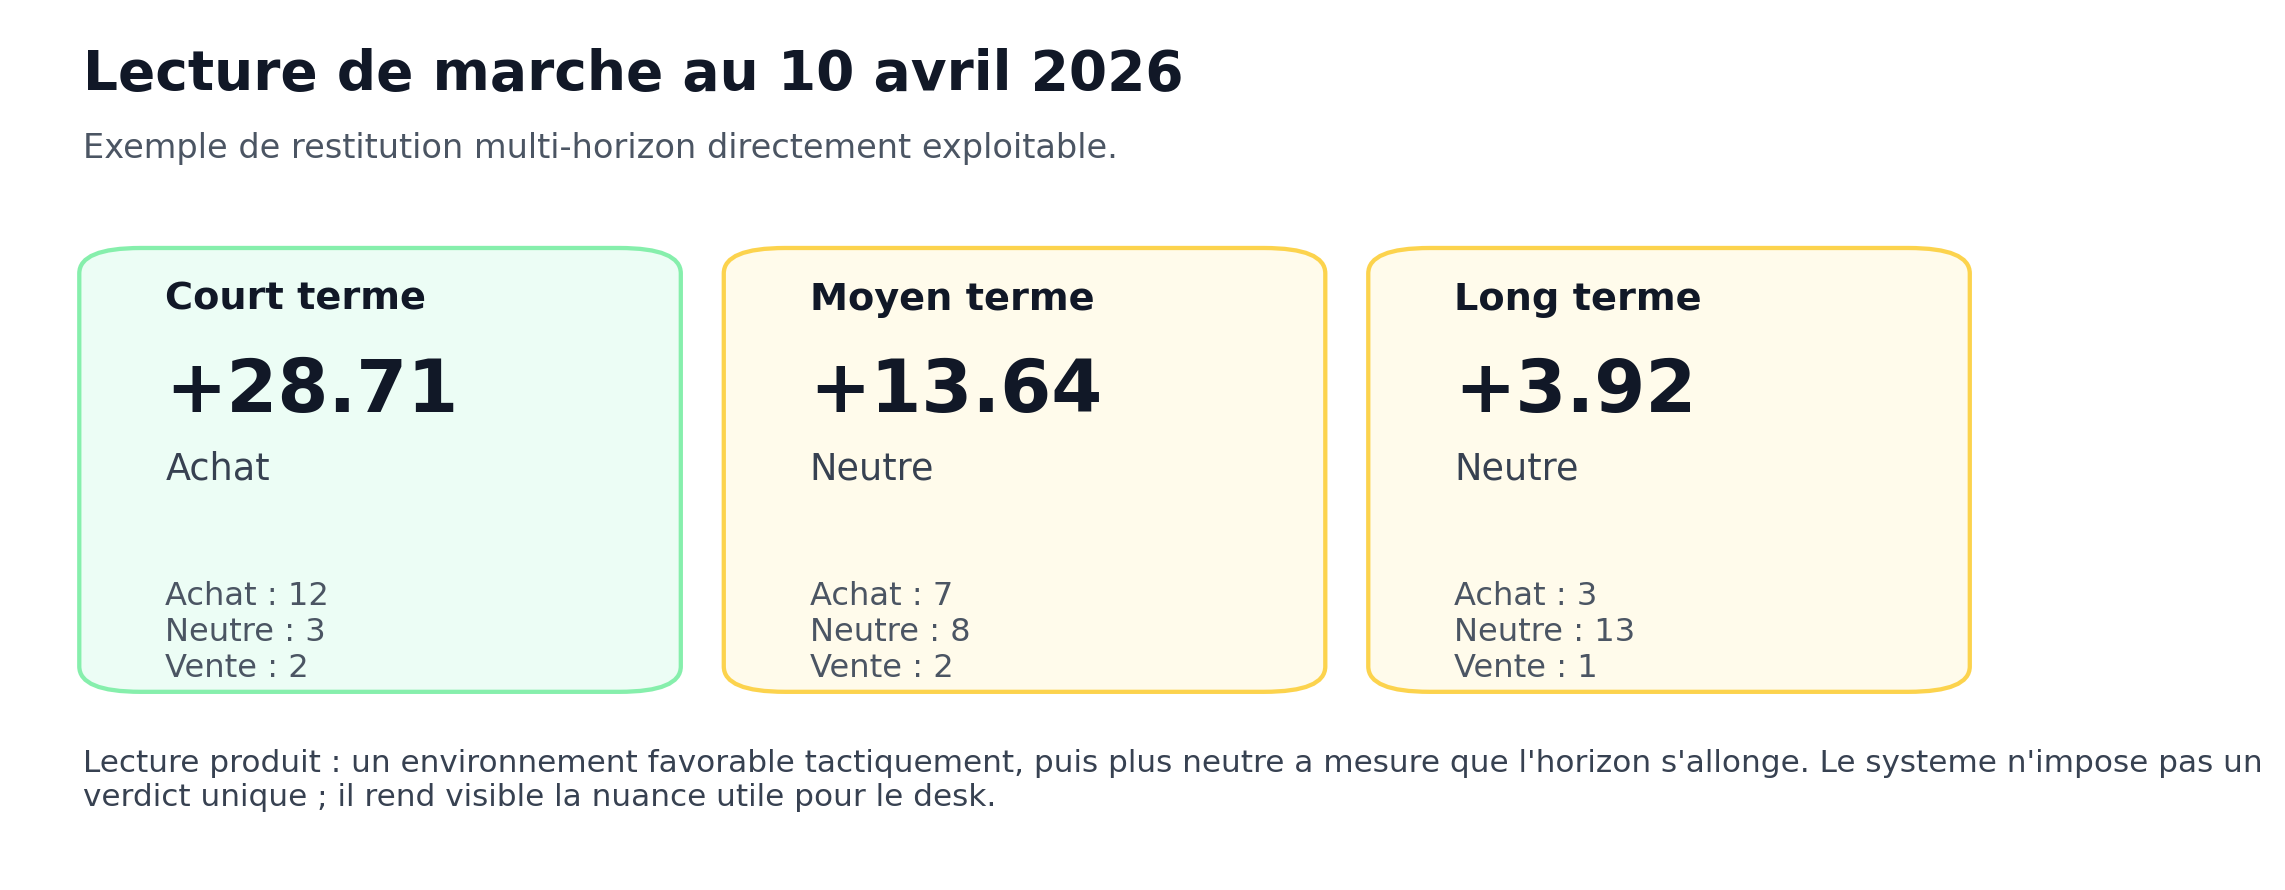
\includegraphics[width=\textwidth]{figures/desk_signal_exec/market_snapshot.png}
\caption{Exemple de lecture de marché par horizon.}
\end{figure}

Le signal de marché ressort en \textbf{Achat} à court terme, puis devient plus \textbf{Neutre} à moyen et long terme. Pour le desk, ce point est utile : le produit aide à voir où les opportunités paraissent les plus fortes, sans masquer la nuance selon l'horizon.

\begin{figure}[H]
\centering
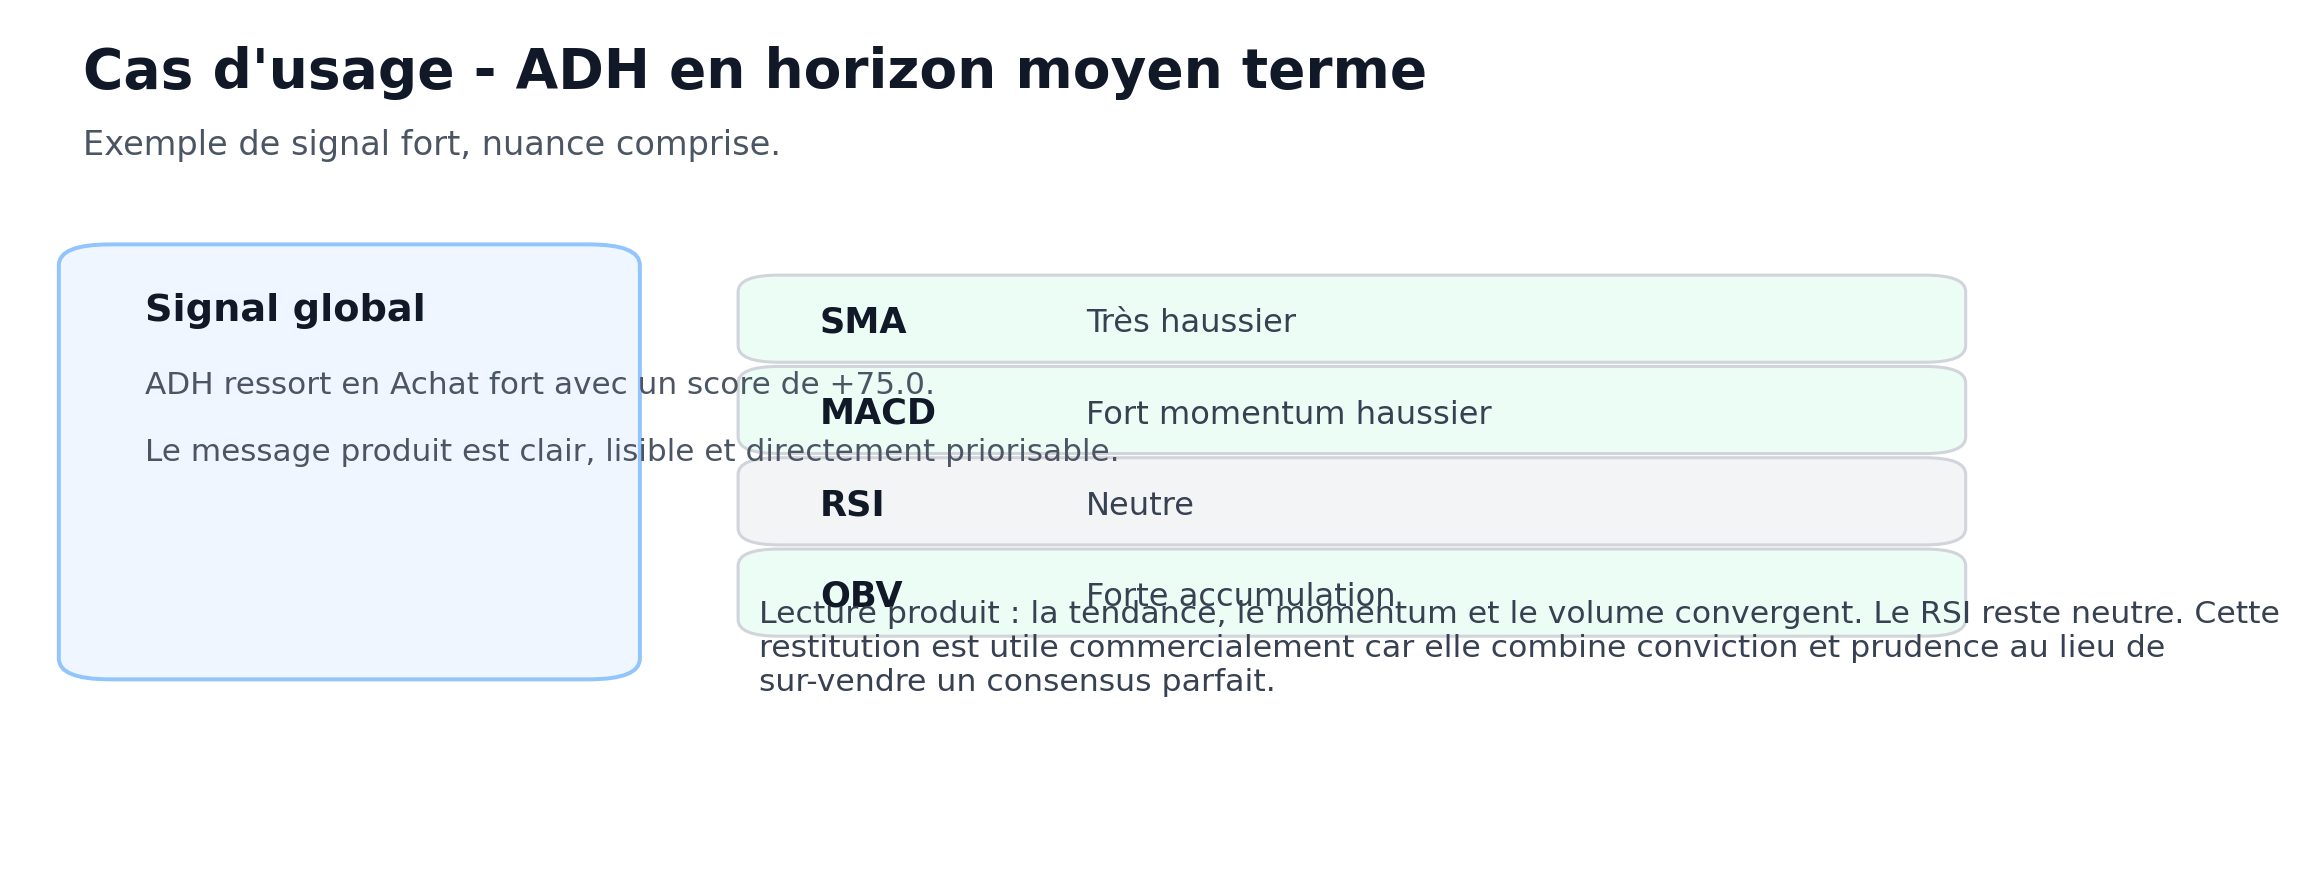
\includegraphics[width=\textwidth]{figures/desk_signal_exec/case_study_adh.png}
\caption{Cas d'usage : lecture produit sur ADH en moyen terme.}
\end{figure}

Sur le cas \textbf{ADH}, le produit met en avant une lecture forte sans masquer la nuance. La tendance, le momentum et le volume convergent. Le RSI, lui, reste neutre. Cette présentation est plus crédible commercialement qu'un affichage uniforme : elle inspire davantage confiance parce qu'elle n'exagère pas le signal.

\section*{5. Valeur ajoutée pour le desk}

La valeur du produit tient à cinq points.

\textbf{Premièrement,} il aide à trouver plus vite les titres qui ressortent réellement.

\textbf{Deuxièmement,} il réduit la dispersion analytique. Le desk ne part plus de lectures isolées et hétérogènes ; il part d'une base commune.

\textbf{Troisièmement,} il améliore la vitesse de lecture. Le dashboard fait ressortir les titres et les segments qui méritent une attention immédiate.

\textbf{Quatrièmement,} il renforce l'explicabilité. Quand un titre ressort, le desk peut revenir au détail au lieu de s'arrêter à une étiquette.

\textbf{Cinquièmement,} il crédibilise la lecture technique. Le recours à une logique de robustesse et d'évaluation hors échantillon réduit le risque de conclusions trop opportunistes.

Au fond, le produit ne vend pas un miracle. Il apporte quelque chose de plus utile pour un desk : \textbf{un moyen plus clair et plus rapide d'identifier les meilleures opportunités du marché}.

\section*{6. Limites et perspectives}

Le produit est utile dans son périmètre actuel, mais il doit être présenté avec sobriété.

\begin{itemize}
\item Le cœur publié est centré sur quatre familles ; cela favorise la clarté, mais reste volontairement resserré.
\item La qualité du signal dépend de la qualité et de la fraîcheur des données.
\item Le produit reste une \textbf{brique d'aide à l'analyse}, pas un moteur d'exécution.
\end{itemize}

Les perspectives les plus naturelles sont déjà identifiées :

\begin{itemize}
\item élargir progressivement l'univers d'indicateurs ;
\item enrichir encore la restitution visuelle ;
\item renforcer les vues de comparaison entre titres, secteurs et horizons.
\end{itemize}

\vspace{0.7em}
\fcolorbox{black}{gray!8}{
\parbox{0.96\textwidth}{
\textbf{Message clé.} Le produit présenté aide les traders du desk à trouver les meilleures opportunités du marché. Le moteur structure l'information, la page Signals l'explique et le dashboard la transforme en lecture immédiatement exploitable.
}}

\end{document}
